%In this subsection we derive the basis for the Argyris element using the
%standard Cartesian coordinates on a reference triangle $\hat{K}$ as opposed to
%the area coordinates on a general triangle $K$ as used by \cite{Okabe}.
%The transformation developed by \cite{Dominguez08}, which will be discussed in \autoref{sse:Trans}, allows for all computations to be done on the reference triangle
%and so the bulk of the discussion will be concerned with developing the basis
%functions on $\hat{K}$ and the transformation.
\begin{figure}%[H]
	\begin{center}
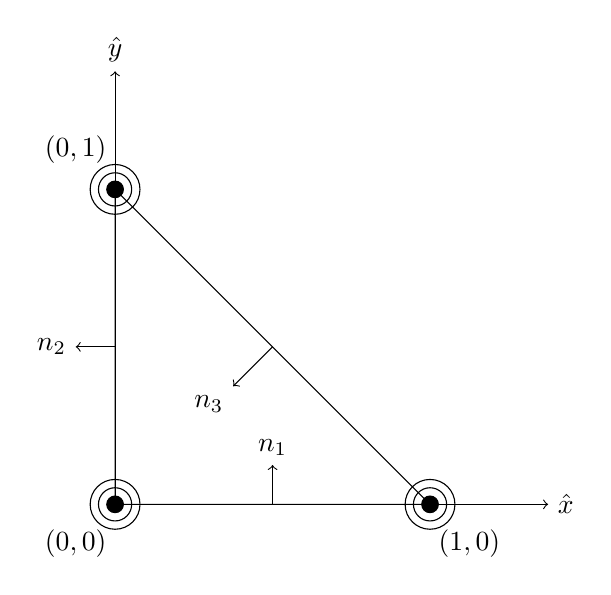
\begin{tikzpicture}
  %draw the axes
  \draw[->] (0,0) -- (5.5,0) node[right,fill=none] {$\hat{x}$};
  \draw[->] (0,0) -- (0,5.5) node[above,fill=none] {$\hat{y}$};
  %draw the triangle
	\draw (0,0) -- (4,0) -- (0,4) -- cycle;
	%draw the interpolation points
	%function values
	\filldraw (0,0) circle(3pt);
	\filldraw (4,0) circle(3pt);
	\filldraw (0,4) circle(3pt);
	%first derivatives
	\draw (0,0) circle(6pt);
	\draw (4,0) circle(6pt);
	\draw (0,4) circle(6pt);
	%second derivatives
	\draw (0,0) circle(9pt);
	\draw (4,0) circle(9pt);
	\draw (0,4) circle(9pt);
	%normal derivatives
  \draw[->] (2,0) -- (2,0.5) node[above,fill=none] {$n_1$};
  \draw[->] (0,2) -- (-0.5,2) node[left,fill=none] {$n_2$};
  \draw[->] (2,2) -- (1.5,1.5) node[below left,fill=none] {$n_3$};
  %label vertices
  %\node[circle] at (-0.6,0) {$1$};
  %\node at (4,-0.6) {$2$};
  %\node at (-0.6,4) {$3$};
  \node at (-0.5,-0.5) {$(0,0)$};
  \node at (4.5,-0.5) {$(1,0)$};
  \node at (-0.5,4.5) {$(0,1)$};
\end{tikzpicture}
	\end{center}
  \caption{The reference triangle $\hat{K}$ for the Argyris element.}
	\label{fig:RefTriangle}
\end{figure}


The Argyris triangle has 21 degrees of freedom and therefore has 21 basis functions per triangle.
Additionally, the basis for Argyris in reference coordinates (depicted in \autoref{fig:RefTriangle})
belong to the space $\mathbb{P}_5$, which has the standard monomial basis
\begin{equation*}
	\left\{
    1, x, y, x^2, xy, y^2, x^3, x^2y, xy^2, y^3, x^4, x^3y, 
    x^2y^2, xy^3, y^4, x^5, x^4y, x^3y^2, x^2y^3, xy^4, y^4 
  \right\}
\end{equation*}
Thus, the $i^{th}$ basis function for the Argyris triangle can be written as 
\begin{equation}
	\begin{split}
	\hat{\varphi}_i(\hat{x},\hat{y}) = m^i_1 + m^i_2 \hat{x} + m^i_3 \hat{x}^2 + m^i_4 \hat{x}^3 + m^i_5 \hat{x}^4 + m^i_6 \hat{x}^5 + m^i_7 \hat{y} + m^i_8
 	\hat{y}^2 + m^i_9 \hat{y}^3 \\
 + m^i_{10} \hat{y}^4 + m^i_{11} \hat{y}^5 + m^i_{12}  \hat{x} \hat{y} + m^i_{13} \hat{x} \hat{y}^2 + m^i_{14} \hat{x} \hat{y}^3 + m^i_{15}
 	\hat{x} \hat{y}^4 + m^i_{16} \hat{x}^2 \hat{y} \\ 
 + m^i_{17} \hat{x}^2 \hat{y}^2 + m^i_{18}\hat{x}^2 \hat{y}^3 + m^i_{19} \hat{x}^3 \hat{y} + m^i_{20}\hat{x}^3 \hat{y}^2 + m^i_{21} \hat{x}^4 \hat{y}
 \end{split}
	\label{eqn:Basis}
\end{equation}

Now, consider the reference triangle $\hat{K}$ in Figure \ref{fig:RefTriangle} with
vertices numbered counter clockwise $1,\, 2,\text{ and } 3$, i.e.
$(\hat{x}_1,\hat{y}_1)=(0,0),\, (\hat{x}_2,\hat{y}_2)=(1,0),\text{ and } (\hat{x}_3,\hat{y}_3)=(0,1)$.
Additionally, let the vector $v_i$ represent the $i^{th}$ edge with
\begin{equation*}
  v_1 = [\hat{x}_2-\hat{x}_1,\hat{y}_2-\hat{y}_1]^T, \quad v_2=[\hat{x}_3-\hat{x}_1,\hat{y}_3-\hat{y}_1]^T \text{ and } v_3=[\hat{x}_3
  -\hat{x}_2,\hat{y}_3-\hat{y}_2]^T.
\end{equation*}
Also, we will use the convention that the $i^{th}$ normal vector is the rotation
of the $v_i$ counter-clockwise $90^\circ$. Therefore, the $i^{th}$ basis
function can be found using the restriction in Table \ref{tab:Constraints}.

\begin{table}%[H]
\begin{center}
  {\tiny\begin{tabular}{|p{1.2in}|p{1.2in}|p{1.2in}|}
	\hline
	$i,j,k=1,2,3$ & $i=4,5,6$ and $j,k=1,2,3$ &
	$i=7,8,9$ and $j,k=1,2,3$ \\
	\hline
	\begin{equation*}
		\begin{split}
		\varphi_i (x_j,y_j) = \delta_{i,j} \\
		\dfrac{\partial \varphi_i}{\partial x} (x_j,y_j) = 0 \\
		\dfrac{\partial \varphi_i}{\partial y} (x_j,y_j) = 0 \\
		\dfrac{\partial^2 \varphi_i}{\partial x^2} (x_j,y_j) = 0 \\
		\dfrac{\partial^2 \varphi_i}{\partial x \partial y} (x_j,y_j) = 0 \\
		\dfrac{\partial^2 \varphi_i}{\partial y^2} (x_j,y_j) = 0 \\
		\dfrac{\partial\varphi_i}{\partial n_k} = 0
		\end{split}
	\end{equation*} &
	\begin{equation*}
		\begin{split}
		\varphi_i (x_j,y_j) = 0 \\
		\dfrac{\partial \varphi_i}{\partial x} (x_j,y_j) = \delta_{i,j+3} \\
		\dfrac{\partial \varphi_i}{\partial y} (x_j,y_j) = 0 \\
		\dfrac{\partial^2 \varphi_i}{\partial x^2} (x_j,y_j) = 0 \\
		\dfrac{\partial^2 \varphi_i}{\partial x \partial y} (x_j,y_j) = 0 \\
		\dfrac{\partial^2 \varphi_i}{\partial y^2} (x_j,y_j) = 0 \\
		\dfrac{\partial\varphi_i}{\partial n_k} = 0
		\end{split}
	\end{equation*} &
	\begin{equation*}
		\begin{split}
		\varphi_i (x_j,y_j) = 0 \\
		\dfrac{\partial \varphi_i}{\partial x} (x_j,y_j) = 0 \\
		\dfrac{\partial \varphi_i}{\partial y} (x_j,y_j) = \delta_{i,j+6} \\
		\dfrac{\partial^2 \varphi_i}{\partial x^2} (x_j,y_j) = 0 \\
		\dfrac{\partial^2 \varphi_i}{\partial x \partial y} (x_j,y_j) = 0 \\
		\dfrac{\partial^2 \varphi_i}{\partial y^2} (x_j,y_j) = 0 \\
		\dfrac{\partial\varphi_i}{\partial n_k} = 0
		\end{split}
	\end{equation*} \\
	\hline
	\hline
	$i=10,11,12$ and $j,k=1,2,3$
	& $i=13,14,15$ and $j,k=1,2,3$ &
	$i=16,17,18$ and $j,k=1,2,3$ \\
	\hline
	\begin{equation*}
		\begin{split}
		\varphi_i (x_j,y_j) = 0 \\
		\dfrac{\partial \varphi_i}{\partial x} (x_j,y_j) = 0 \\
		\dfrac{\partial \varphi_i}{\partial y} (x_j,y_j) = 0 \\
		\dfrac{\partial^2 \varphi_i}{\partial x^2} (x_j,y_j) = \delta_{i,j+9} \\
		\dfrac{\partial^2 \varphi_i}{\partial x \partial y} (x_j,y_j) = 0 \\
		\dfrac{\partial^2 \varphi_i}{\partial y^2} (x_j,y_j) = 0 \\
		\dfrac{\partial\varphi_i}{\partial n_k} = 0
		\end{split}
	\end{equation*} &
	\begin{equation*}
		\begin{split}
		\varphi_i (x_j,y_j) = 0 \\
		\dfrac{\partial \varphi_i}{\partial x} (x_j,y_j) = 0 \\
		\dfrac{\partial \varphi_i}{\partial y} (x_j,y_j) = 0 \\
		\dfrac{\partial^2 \varphi_i}{\partial x^2} (x_j,y_j) = 0 \\
		\dfrac{\partial^2 \varphi_i}{\partial x \partial y} (x_j,y_j) = 0 \\
		\dfrac{\partial^2 \varphi_i}{\partial y^2} (x_j,y_j) = \delta_{i,j+12} \\
		\dfrac{\partial\varphi_i}{\partial n_k} = 0
		\end{split}
	\end{equation*} &
	\begin{equation*}
		\begin{split}
		\varphi_i (x_j,y_j) = 0 \\
		\dfrac{\partial \varphi_i}{\partial x} (x_j,y_j) = 0 \\
		\dfrac{\partial \varphi_i}{\partial y} (x_j,y_j) = 0 \\
		\dfrac{\partial^2 \varphi_i}{\partial x^2} (x_j,y_j) = 0 \\
		\dfrac{\partial^2 \varphi_i}{\partial x \partial y} (x_j,y_j) = \delta_{i,j+15} \\
		\dfrac{\partial^2 \varphi_i}{\partial y^2} (x_j,y_j) = 0 \\
		\dfrac{\partial\varphi_i}{\partial n_k} = 0
		\end{split}
	\end{equation*} \\
	\hline
	\hline
	& $i=19,20,21$ and $k=1,2,3$ & \\
	\hline
	& \begin{equation*}
		\begin{split}
		\varphi_i (x_j,y_j) = 0 \\
		\dfrac{\partial \varphi_i}{\partial x} (x_j,y_j) = 0 \\
		\dfrac{\partial \varphi_i}{\partial y} (x_j,y_j) = 0 \\
		\dfrac{\partial^2 \varphi_i}{\partial x^2} (x_j,y_j) = 0 \\
		\dfrac{\partial^2 \varphi_i}{\partial x \partial y} (x_j,y_j) = 0 \\
		\dfrac{\partial^2 \varphi_i}{\partial y^2} (x_j,y_j) = 0 \\
		\dfrac{\partial\varphi_i}{\partial n_k} = \delta_{i,k-18}
		\end{split}
	\end{equation*} & \\
	\hline
\end{tabular}}
\caption{Constraints for Argyris triangle
  \cite{Argyris,Brenner,Ciarlet,Dominguez08}}
\label{tab:Constraints}
\end{center}
\end{table}


Now, let $z$ be the vector containing the monomial basis for $\mathbb{P}_5$, i.e.
\small{
\begin{equation*}
  z=\left[
    1, \hat{x}, \hat{y}, \hat{x}^2, \hat{x}\hat{y}, \hat{y}^2, \hat{x}^3, \hat{x}^2\hat{y}, \hat{x}\hat{y}^2, \hat{y}^3, \hat{x}^4, \hat{x}^3\hat{y}, 
    \hat{x}^2\hat{y}^2, \hat{x}\hat{y}^3, \hat{y}^4, \hat{x}^5, \hat{x}^4\hat{y}, \hat{x}^3\hat{y}^2, \hat{x}^2\hat{y}^3, \hat{x}\hat{y}^4, \hat{y}^4 
  \right]^{T}
\end{equation*}}
Then the $i^{th}$ Argyris basis function on $\hat{K}$ is given by
\begin{equation*}
  \hat{\varphi}_i = M_i z,
\end{equation*}
where $M_i$ is the $i^{th}$ row of the matrix $M$. Therefore, the evaluation of
$\hat{\varphi}_i(\hat{x},\hat{y})$ comes down to the matrix-vector multiplication
\begin{equation*}
  \hat{\varphi}_i(\hat{x},\hat{y}) = M_i z(\hat{x},\hat{y}).
\end{equation*}

To determine the matrix $M$ we must solve the linear system 
\begin{equation*}
  ZM^T=I_{21}
\end{equation*}
that result from the constraints in Table \ref{tab:Constraints}. Here
\begin{equation*}
  \begin{split}Z=[z(0,0), z(0,1), z(1,0), 
  z_{\hat{x}}(0,0), z_{\hat{y}}(0,0), 
  z_{\hat{x}}(1,0), z_{\hat{y}}(1,0), 
  z_{\hat{x}}(0,1), z_{\hat{y}}(0,1), \\
  z_{\hat{x}\hat{x}}(0,0), z_{\hat{x}\hat{y}}(0,0), z_{\hat{y}\hat{y}}(0,0), 
  z_{\hat{x}\hat{x}}(1,0), z_{\hat{x}\hat{y}}(1,0), z_{\hat{y}\hat{y}}(1,0), \\
  z_{\hat{x}\hat{x}}(0,1), z_{\hat{x}\hat{y}}(0,1), z_{\hat{y}\hat{y}}(0,1), 
  z_{\hat{y}}(\nicefrac{1}{2},0), -z_{\hat{x}}(0,\nicefrac{1}{2}), \\
  -\frac{1}{\sqrt{2}}(z_{\hat{x}}(\nicefrac{1}{2},\nicefrac{1}{2}) +
  z_{\hat{y}}(\nicefrac{1}{2},\nicefrac{1}{2}))]^T\end{split}
\end{equation*}
$I_{21}$ is a $21\times 21$ identity matrix and $M$ is the matrix containing the
coefficients for all 21 basis functions. Therefore solving this system will
result in a matrix, $M$, that contains the coefficients for the Argyris basis
functions for the reference triangle as in \eqref{eqn:Basis}. Thus, the matrix
$M$ is \\ 
%\begin{sideways}
%\begin{minipage}[h]{0.7\textheight}
%  \vspace{0.25\textwidth}
\begin{sidewaystable}%[H]
  \begin{center}
{\small%tiny
\begin{equation*}
 \left[\begin{array}{ccccccccccccccccccccc}
1 & 0 & 0 & 0 & 0 & 0 & -10 & 0 & 0 & -10 & 15 & 0 & -30 & 0 & 15 & -6 & 0 & 30 & 30 & 0 & -6 \\[0.5em]
0 & 0 & 0 & 0 & 0 & 0 & 10 & 0 & 0 & 0 & -15 & 0 & 15 & 0 & 0 & 6 & 0 & -15 & -15 & 0 & 0 \\[0.5em]
0 & 0 & 0 & 0 & 0 & 0 & 0 & 0 & 0 & 10 & 0 & 0 & 15 & 0 & -15 & 0 & 0 & -15 & -15 & 0 & 6 \\[0.5em]
0 & 1 & 0 & 0 & 0 & 0 & -6 & 0 & -11 & 0 & 8 & 0 & 10 & 18 & 0 & -3 & 0 & 1 & -10 & -8 & 0 \\[0.5em]
0 & 0 & 1 & 0 & 0 & 0 & 0 & -11 & 0 & -6 & 0 & 18 & 10 & 0 & 8 & 0 & -8 & -10 & 1 & 0 & -3 \\[0.5em]
0 & 0 & 0 & 0 & 0 & 0 & -4 & 0 & 0 & 0 & 7 & 0 & -\frac{7}{2} & 0 & 0 & -3 & 0 & \frac{7}{2} & \frac{7}{2} & 0 & 0 \\[0.5em]
0 & 0 & 0 & 0 & 0 & 0 & 0 & -5 & 0 & 0 & 0 & 14 & \frac{37}{2} & 0 & 0 & 0 & -8 & -\frac{37}{2} & -\frac{27}{2} & 0 & 0 \\[0.5em]
0 & 0 & 0 & 0 & 0 & 0 & 0 & 0 & -5 & 0 & 0 & 0 & \frac{37}{2} & 14 & 0 & 0 & 0 & -\frac{27}{2} & -\frac{37}{2} & -8 & 0 \\[0.5em]
0 & 0 & 0 & 0 & 0 & 0 & 0 & 0 & 0 & -4 & 0 & 0 & -\frac{7}{2} & 0 & 7 & 0 & 0 & \frac{7}{2} & \frac{7}{2} & 0 & -3 \\[0.5em]
0 & 0 & 0 & \frac{1}{2} & 0 & 0 & -\frac{3}{2} & 0 & 0 & 0 & \frac{3}{2} & 0 & -\frac{3}{2} & 0 & 0 & -\frac{1}{2} & 0 & \frac{3}{2} & 1 & 0 & 0 \\[0.5em]
0 & 0 & 0 & 0 & 1 & 0 & 0 & -4 & -4 & 0 & 0 & 5 & 10 & 5 & 0 & 0 & -2 & -6 & -6 & -2 & 0 \\[0.5em]
0 & 0 & 0 & 0 & 0 & \frac{1}{2} & 0 & 0 & 0 & -\frac{3}{2} & 0 & 0 & -\frac{3}{2} & 0 & \frac{3}{2} & 0 & 0 & 1 & \frac{3}{2} & 0 & -\frac{1}{2} \\[0.5em]
0 & 0 & 0 & 0 & 0 & 0 & \frac{1}{2} & 0 & 0 & 0 & -1 & 0 & \frac{1}{4} & 0 & 0 & \frac{1}{2} & 0 & -\frac{1}{4} & -\frac{1}{4} & 0 & 0 \\[0.5em]
0 & 0 & 0 & 0 & 0 & 0 & 0 & 1 & 0 & 0 & 0 & -3 & -\frac{7}{2} & 0 & 0 & 0 & 2 & \frac{7}{2} & \frac{5}{2} & 0 & 0 \\[0.5em]
0 & 0 & 0 & 0 & 0 & 0 & 0 & 0 & 0 & 0 & 0 & 0 & \frac{5}{4} & 0 & 0 & 0 & 0 & -\frac{3}{4} & -\frac{5}{4} & 0 & 0 \\[0.5em]
0 & 0 & 0 & 0 & 0 & 0 & 0 & 0 & 0 & 0 & 0 & 0 & \frac{5}{4} & 0 & 0 & 0 & 0 & -\frac{5}{4} & -\frac{3}{4} & 0 & 0 \\[0.5em]
0 & 0 & 0 & 0 & 0 & 0 & 0 & 0 & 1 & 0 & 0 & 0 & -\frac{7}{2} & -3 & 0 & 0 & 0 & \frac{5}{2} & \frac{7}{2} & 2 & 0 \\[0.5em]
0 & 0 & 0 & 0 & 0 & 0 & 0 & 0 & 0 & \frac{1}{2} & 0 & 0 & \frac{1}{4} & 0 & -1 & 0 & 0 & -\frac{1}{4} & -\frac{1}{4} & 0 & \frac{1}{2} \\[0.5em]
0 & 0 & 0 & 0 & 0 & 0 & 0 & 16 & 0 & 0 & 0 & -32 & -32 & 0 & 0 & 0 & 16 & 32 & 16 & 0 & 0 \\[0.5em]
0 & 0 & 0 & 0 & 0 & 0 & 0 & 0 & -16 & 0 & 0 & 0 & 32 & 32 & 0 & 0 & 0 & -16 & -32 & -16 & 0 \\[0.5em]
0 & 0 & 0 & 0 & 0 & 0 & 0 & 0 & 0 & 0 & 0 & 0 & 8\sqrt{2} & 0 & 0 & 0 & 0 & -8\sqrt{2} & -8\sqrt{2} & 0 & 0
  \end{array}\right]
\end{equation*}
}
\caption{Coefficients for the Argyris basis matrix, $M$.}
\label{tab:Coefficients}
  \end{center}
\end{sidewaystable}
%\end{minipage}
%\end{sideways} \\


Therefore, the Argyris basis functions are
\begin{equation}
\begin{split}
  \hat{\varphi}_1(\hat{x},\hat{y}) &= 1-10\hat{x}^3-10\hat{y}^3+15\hat{x}^4-30\hat{x}^2\hat{y}^2+15\hat{y}^4-6\hat{x}^5+30\hat{x}^3\hat{y}^2+30\hat{x}^2\hat{y}^3-6\hat{y}^5 \\
  \hat{\varphi}_2(\hat{x},\hat{y}) &= 10\hat{x}^3-15\hat{x}^4+15\hat{x}^2\hat{y}^2+6\hat{x}^5-15\hat{x}^3\hat{y}^2-15\hat{x}^2\hat{y}^3 \\
  \hat{\varphi}_3(\hat{x},\hat{y}) &= 10\hat{y}^3+15\hat{x}^2\hat{y}^2-15\hat{y}^4-15\hat{x}^3\hat{y}^2-15\hat{x}^2\hat{y}^3+6\hat{y}^2 \\
  \hat{\varphi}_4(\hat{x},\hat{y}) &= \hat{x}-6\hat{x}^3-11\hat{x}\hat{y}^2+8\hat{x}^4+10\hat{x}^2\hat{y}^2+18\hat{x}\hat{y}^3-3\hat{x}^5+\hat{x}^3\hat{y}^2-10\hat{x}^2\hat{y}^3-8\hat{x}\hat{y}^4 \\
  \hat{\varphi}_5(\hat{x},\hat{y}) &= \hat{y}-11\hat{x}^2\hat{y}-6\hat{y}^3+18\hat{x}^3\hat{y}+10\hat{x}^2\hat{y}^2+8\hat{y}^4-8\hat{x}^4\hat{y}-10\hat{x}^3\hat{y}^2+\hat{x}^2\hat{y}^3-3\hat{y}^5 \\
  \hat{\varphi}_6(\hat{x},\hat{y}) &= -4\hat{x}^3+7\hat{x}^4-\frac{7}{2}\hat{x}^2\hat{y}^2-3\hat{x}^5+\frac{7}{2}\hat{x}^3\hat{y}^2+\frac{7}{2}\hat{x}^2\hat{y}^3 \\
  \hat{\varphi}_7(\hat{x},\hat{y}) &= -5\hat{x}^2\hat{y}+14\hat{x}^3\hat{y}+\frac{37}{2}\hat{x}^2\hat{y}^2-8\hat{x}^4\hat{y}-\frac{37}{2}\hat{x}^3\hat{y}^2-\frac{27}{2}\hat{x}^2\hat{y}^3 \\
  \hat{\varphi}_8(\hat{x},\hat{y}) &= -5\hat{x}\hat{y}^2+\frac{37}{2}\hat{x}^2\hat{y}^2+14\hat{x}\hat{y}^3-\frac{27}{2}\hat{x}^3\hat{y}^2-\frac{37}{2}\hat{x}^3\hat{y}^2-8\hat{x}\hat{y}^4 \\
  \hat{\varphi}_9(\hat{x},\hat{y}) &= -4\hat{y}^3-\frac{7}{2}\hat{x}^3+7\hat{y}^4+\frac{7}{2}\hat{x}^3\hat{y}^2+\frac{7}{2}\hat{x}^2\hat{y}^3-3\hat{y}^5 \\
  \hat{\varphi}_{10}(\hat{x},\hat{y}) &= \frac{1}{2}\hat{x}^2-\frac{3}{2}\hat{x}^3+\frac{3}{2}\hat{x}^4-\frac{3}{2}\hat{x}^2\hat{y}^2-\frac{1}{2}\hat{x}^5+\frac{3}{2}\hat{x}^3\hat{y}^2+\hat{x}^2\hat{y}^3 \\
  \hat{\varphi}_{11}(\hat{x},\hat{y}) &= \hat{x}\hat{y}-4\hat{x}^2\hat{y}-4\hat{x}\hat{y}^2+5\hat{x}^3\hat{y}+10\hat{x}^2\hat{y}^2+5\hat{x}\hat{y}^3-2\hat{x}^4\hat{y}-6\hat{x}^3\hat{y}^2-6\hat{x}^2\hat{y}^3-2\hat{x}\hat{y}^4 \\
  \hat{\varphi}_{12}(\hat{x},\hat{y}) &= \frac{1}{2}\hat{y}^2-\frac{3}{2}\hat{y}^3-\frac{3}{2}\hat{x}^2\hat{y}^2+\frac{3}{2}\hat{y}^4+\hat{x}^3\hat{y}^2+\frac{3}{2}\hat{x}^2\hat{y}^3-\frac{1}{2}\hat{y}^5 \\
  \hat{\varphi}_{13}(\hat{x},\hat{y}) &= \frac{1}{2}\hat{x}^3-\hat{x}^4+\frac{1}{4}\hat{x}^2\hat{y}^2+\frac{1}{2}\hat{x}^5-\frac{1}{4}\hat{x}^3\hat{y}^2-\frac{1}{4}\hat{x}^2\hat{y}^3 \\
  \hat{\varphi}_{14}(\hat{x},\hat{y}) &= \hat{x}^2\hat{y}-3\hat{x}^3\hat{y}-\frac{7}{2}\hat{x}^2\hat{y}^2+2\hat{x}^4\hat{y}+\frac{7}{2}\hat{x}^3\hat{y}^2+\frac{5}{2}\hat{x}^2\hat{y}^3 \\
  \hat{\varphi}_{15}(\hat{x},\hat{y}) &= \frac{5}{4}\hat{x}^2\hat{y}^2-\frac{3}{4}\hat{x}^3\hat{y}^2-\frac{5}{4}\hat{x}^2\hat{y}^3 \\
  \hat{\varphi}_{16}(\hat{x},\hat{y}) &= \frac{5}{4}\hat{x}^2\hat{y}^2-\frac{5}{4}\hat{x}^3\hat{y}^2-\frac{3}{4}\hat{x}^2\hat{y}^3 \\
  \hat{\varphi}_{17}(\hat{x},\hat{y}) &= \hat{x}\hat{y}^2-\frac{7}{2}\hat{x}^2\hat{y}^2-3\hat{x}\hat{y}^3+\frac{5}{2}\hat{x}^3\hat{y}^2+\frac{7}{2}\hat{x}^2\hat{y}^3+2\hat{x}\hat{y}^4 \\
  \hat{\varphi}_{18}(\hat{x},\hat{y}) &= \frac{1}{2}\hat{y}^3+\frac{1}{4}\hat{x}^2\hat{y}^2-\hat{y}^4-\frac{1}{4}\hat{x}^3\hat{y}^2-\frac{1}{4}\hat{x}^2\hat{y}^3+\frac{1}{2}\hat{y}^5 \\
  \hat{\varphi}_{19}(\hat{x},\hat{y}) &= 16\hat{x}^2\hat{y}-32\hat{x}^3\hat{y}-32\hat{x}^2\hat{y}^2+16\hat{x}^4\hat{y}+32\hat{x}^3\hat{y}^2+16\hat{x}^2\hat{y}^3 \\
  \hat{\varphi}_{20}(\hat{x},\hat{y}) &= -16\hat{x}\hat{y}^2+32\hat{x}^2\hat{y}^2+32\hat{x}\hat{y}^3-16\hat{x}^3\hat{y}^2-32\hat{x}^2\hat{y}^3-16\hat{x}\hat{y}^4 \\
  \hat{\varphi}_{21}(\hat{x},\hat{y}) &= \sqrt{2}\left(8\hat{x}^2\hat{y}^2-8\hat{x}^3\hat{y}^2-8\hat{x}^2\hat{y}^3\right)
\end{split}
\label{eqn:Argyris}
\end{equation}



